\chapter{Introducción teórica a fuentes CC}
% ----------------------

\label{C:Fuentes de corriente continua}

\section{Sobre las fuentes de alimentación.} \par
Las fuentes de alimentación electrónicas se definen como circuitos que transforman la potencia eléctrica de entrada, ya sea de corriente alterna (CA) o de corriente continua (CC), en potencia de salida, ya sea de corriente alterna (CA) o de corriente continua (CC). Esta definición excluye así a las fuentes de alimentación basadas en los principios de máquinas rotativas y distingue las fuentes de alimentación de la categoría más general de fuentes de energía eléctrica que derivan la potencia eléctrica de otras formas de energía (por ejemplo, baterías, celdas solares, celdas de combustible). Las fuentes de alimentación electrónicas se pueden dividir en cuatro amplias clasificaciones:

\begin{enumerate}
    \item CA de entrada, CA de salida regulada por línea o cambiadores de frecuencia.
    \item CC de entrada, CC de salida convertida o regulada.
    \item CC de entrada, CA de salida de corriente alterna, conocidas como inversores.
    \item CA de entrada, CC de salida. conocidas como rectificadores.
\end{enumerate}

Esta última categoría es, con mucho, la más común de las cuatro y generalmente es a la que se hace referencia cuando se habla de una "fuente de alimentación". Las fuentes de alimentación de CC de salida pueden proporcionar cuatro salidas básicas o modos de operación:

\begin{itemize}
    \item Voltaje Constante: El voltaje de salida se mantiene constante a pesar de los cambios en la carga, la línea o la temperatura.
    \item Corriente Constante: La corriente de salida se mantiene constante a pesar de los cambios en la carga, la línea o la temperatura.
    \item Límite de Voltaje: Igual que el voltaje constante excepto por características de regulación menos precisas.
    \item Límite de Corriente: Similar a la corriente constante excepto por una regulación menos precisa.
\end{itemize} \par 
Como se explica en esta sección, las fuentes de alimentación están diseñadas para ofrecer estas salidas en diversas combinaciones para diferentes aplicaciones. \cite{agilent2000}. \par 
La analizada en este informe será una fuente con entrada CA y salida CC con control de voltaje y límite de corriente.

\subsection{Fuente ideal de  tensión.} \par 
No existe tal cosa como un dispositivo perfecto en la electrónica, sin embargo con el fin de buscar la excelencia en el diseño y producción de un prototipo de fuente se parte del principio de que características debería presentar la misma para estar lo más próxima a este escenario hipotético. Todo esto lleva a decir que una fuente de alimentación de voltaje constante ideal sería aquella que tendría una impedancia de salida cero en todas las frecuencias. Por lo tanto, el voltaje permanece perfectamente constante a pesar de cualquier cambio en la corriente de salida demandada por la carga. \par 
Una simple fuente de alimentación no regulada compuesta únicamente por un rectificador y un filtro no es capaz de proporcionar un voltaje de salida de corriente continua sin ondulaciones cuyo valor permanece razonablemente constante. Para obtener siquiera una aproximación básica de la característica de salida ideal, algún tipo de elemento de control (regulador) debe incluirse en la fuente. \cite{agilent2000}. 

\begin{figure}
    \centering
    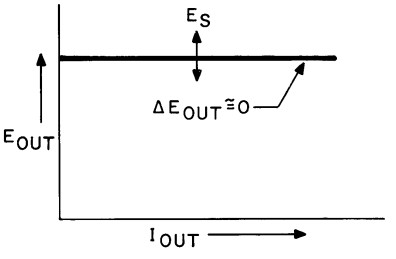
\includegraphics[scale=0.5]{./imagenes/salidaidealfuentedc.jpg}
    \caption{Voltaje de tensión constante salida de fuente ideal.}
    \label{F:salidaidealfuentedc}
\end{figure}

\subsection{Técnicas de Regulación}\par 
La mayoría de las fuentes de alimentación de voltaje constante actuales emplean una de estas cuatro técnicas de regulación:
\begin{itemize}
    \item Serie (Lineal).
    \item Pre-regulador/Regulador en Serie.
    \item Conmutación.
    \item SCR.
\end{itemize}\par 

El objetivo principal de este documento no es proporcionar una explicación exhaustiva de cada uno de estos modelos. En su lugar, se hará una mención breve de todos ellos y se identificará específicamente el modelo que tiene mayor relevancia para los fines de este estudio. Esta aproximación permitirá centrar el análisis en el modelo más pertinente, sin desviar la atención hacia detalles que, aunque importantes, no son esenciales para los propósitos de este trabajo.


\subsection{Fuentes de alimentación lineales.} \par 
Las fuentes de alimentación lineales son un elemento fundamental en la mayoría de los dispositivos electrónicos que utilizamos en nuestra vida cotidiana. Estas fuentes convierten la energía de la red eléctrica en una forma estable y utilizable, proporcionando la energía necesaria para el funcionamiento de los circuitos electrónicos. \par
Una fuente de alimentación lineal consta de varios componentes básicos, como el transformador, el rectificador, el filtro y el regulador de voltaje. Cada uno de estos elementos juega un papel fundamental en garantizar que la energía suministrada sea constante y adecuada para los dispositivos electrónicos, asegurando su correcto funcionamiento.

\section{Funcionamiento básico.} \par 
El tipo más simple y común de fuentes de alimentación de corriente continua (CC) es un sistema \entreComillas{lineal} , mostrado esquemáticamente en la Figura \ref{F:componentesFL}. Primero, se utiliza un transformador para \entreComillas{reducir} la tensión de línea de CA a un voltaje pico más pequeño, que generalmente es aproximadamente 3 voltios superior que el voltaje de salida de CC deseado. Luego, un circuito de diodos rectifica la señal de CA, produciendo una forma de onda con una gran componente de CC. Seguidamente, se utiliza un banco de filtros de condensadores para \entreComillas{suavizar} o \entreComillas{filtrar} la sinusoidal rectificada. \par 
Bajo condiciones de carga normales, siempre hay alguna variación periódica residual o \entreComillas{ripple} en la señal filtrada. Si la aplicación requiere un ripple muy bajo y una salida de CC constante sobre un amplio rango de condiciones de carga, entonces se requiere regulación activa para reducir o eliminar aún más este ripple residual. \cite{tektronix_pws4305}
\begin{figure}
    \centering
    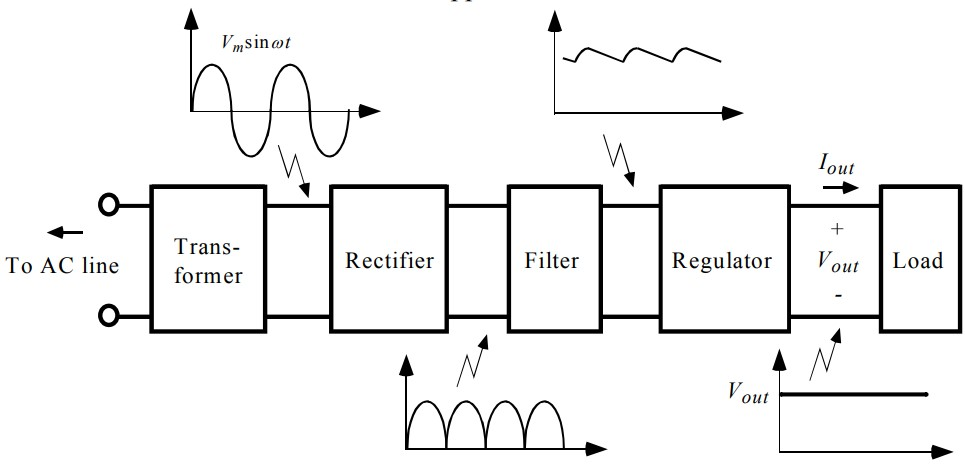
\includegraphics[scale=0.5]{./imagenes/componentesFL.jpg}
    \caption{Diagrama de bloques de una fuente de tensión.}
    \label{F:componentesFL}
\end{figure}

\subsection{Transformador}\par 
El transformador es uno de los componentes principales de una fuente de alimentación lineal. Su función principal es transformar la corriente alterna (CA) de la red eléctrica en una corriente alterna con un voltaje específico adecuado para la aplicación. Consiste en dos bobinas de alambre enrolladas alrededor de un núcleo de hierro, donde la relación entre el número de vueltas en las bobinas determina la relación de transformación del voltaje.

\subsection{Rectificador}\par 
El rectificador es otro componente esencial que convierte la corriente alterna en corriente continua (CC). Esto se logra mediante diodos rectificadores, que permiten que la corriente fluya en una sola dirección. Los rectificadores pueden ser de media onda o de onda completa, dependiendo de cómo se utilizan los diodos para rectificar la señal de entrada.

\subsection{Filtro}\par 
Después de que el rectificador convierte la corriente alterna en corriente continua, la señal resultante puede contener fluctuaciones no deseadas o rizado. Para eliminar estas fluctuaciones y obtener una salida de voltaje suave y constante, se utiliza un filtro. El filtro puede estar compuesto por capacitores y bobinas para eliminar el rizado y suavizar la salida de voltaje.

\subsection{Regulador}\par 
El regulador es el componente final de una fuente de alimentación lineal y se utiliza para mantener constante la salida de voltaje independientemente de las variaciones en la entrada de voltaje o en la carga. Los reguladores de voltaje pueden ser de tipo lineal, que controlan la cantidad de energía disipada como calor para mantener el voltaje de salida constante, o de tipo conmutado, que regulan el voltaje de salida ajustando el ciclo de trabajo de un interruptor.

\section{Ventajas y desventajas}\par 
Todo dispositivo cuenta con una serie de características que la hacen una opción dominante por sobre las demás. Aquí se listan los detalles más dominantes de las fuentes de tensión lineal que las podría hacer sugeribles frente a otro tipo de configuraciones.\par 
\underline{Ventajas}:
\begin{itemize}
    \item Simplicidad: Son relativamente simples en diseño y operación.
    \item Bajo ruido: Tienen un nivel de ruido más bajo en comparación con algunas otras formas de fuentes de alimentación.
    \item Baja interferencia electromagnética (EMI): Emiten menos interferencia electromagnética en comparación con las fuentes de alimentación conmutadas.
    \item Buen rendimiento en aplicaciones de baja potencia: Son eficientes y efectivas en aplicaciones de baja potencia.
    \item Buena regulación: Suelen tener una regulación de voltaje estable y precisa.
\end{itemize}\par 
\underline{Desventajas}:
\begin{itemize}
    \item Baja eficiencia energética: Tienen una eficiencia energética más baja en comparación con las fuentes de alimentación conmutadas, especialmente en aplicaciones de alta potencia.
    \item Disipación de calor: Tienden a generar más calor durante la operación debido a la regulación de voltaje a través de dispositivos de regulación lineal, lo que puede requerir disipadores de calor o ventilación adicional.
    \item Mayor tamaño y peso: Suelen ser más grandes y pesadas en comparación con las fuentes de alimentación conmutadas con la misma capacidad de potencia.
    \item Menor rango de voltaje de entrada: Tienen un rango de voltaje de entrada limitado en comparación con las fuentes de alimentación conmutadas, lo que puede limitar su aplicabilidad en ciertos entornos o condiciones de operación.
\end{itemize}

\section{Evolución y mejoras con el pasar de los años}\par 
Las fuentes de corriente directa (CC) han experimentado una evolución significativa desde sus inicios, impulsadas por avances tecnológicos que han mejorado su eficiencia, fiabilidad y capacidad de adaptación a diversas aplicaciones. A lo largo de los años, estas mejoras han permitido que las fuentes de CC se conviertan en componentes esenciales en una amplia gama de dispositivos electrónicos y sistemas de energía. Las mejoras no solamente abarcan mejores materiales sino también el uso de estrategias de control más inteligentes y adaptación para entornos específicos.\par 
Algunas de estas mejoras son:
\begin{itemize}
    \item \textbf{Tecnología de Conversión de Energía}: Las fuentes de CC modernas utilizan técnicas avanzadas de conversión de energía, como la conmutación de alta frecuencia, que permiten una mayor eficiencia energética y una reducción en el tamaño de los dispositivos. La tecnología de conversión resonante, como los convertidores LLC (Inductor-Inductor-Capacitor), ha mejorado la eficiencia en aplicaciones de alta potencia al minimizar las pérdidas por conmutación \cite{zhang2013}.
    \item \textbf{Materiales de Banda Ancha}: La incorporación de materiales semiconductores de banda ancha, como el carburo de silicio (SiC) y el nitruro de galio (GaN). Estos materiales permiten operar a mayores voltajes y frecuencias, mejorando la eficiencia y reduciendo las pérdidas térmicas. Los dispositivos basados en SiC y GaN son especialmente beneficiosos en aplicaciones de alta potencia y alta densidad \cite{palmour2019}.
    \item \textbf{Integración de Funcionalidades Inteligentes}: Las fuentes de CC actuales incorporan funcionalidades inteligentes, como el monitoreo y control digital en tiempo real, que optimizan el rendimiento y la eficiencia energética. Estas fuentes pueden ajustar dinámicamente sus parámetros de operación en respuesta a las condiciones de carga, mejorando así la fiabilidad y prolongando la vida útil de los componentes conectados \cite{brown2020}.
    \item \textbf{Reducción del Tamaño y Peso}: Los avances en diseño y materiales han permitido la reducción significativa del tamaño y peso de las fuentes de DC. Esto es crucial en aplicaciones donde el espacio es limitado, como en la electrónica de consumo portátil y los vehículos eléctricos. La miniaturización también ha facilitado la integración de fuentes de DC en dispositivos médicos y aplicaciones aeroespaciales \cite{kumar2017}.
    \item \textbf{Energía Renovable y Almacenamiento}: Las fuentes de CC han evolucionado para integrarse de manera más efectiva con sistemas de energía renovable y almacenamiento de energía. Las mejoras en la gestión de energía y la capacidad de interactuar con baterías avanzadas y sistemas de almacenamiento han sido vitales para aplicaciones en redes inteligentes y micro-redes \cite{hoffmann2021}.
\end{itemize}\par 
\section{Fuentes comerciales}\par 
Para aquellos lectores que deseen profundizar más allá del contenido de este informe, los invitamos a explorar diversos tipos de fuentes comerciales disponibles en el mercado. A continuación, presentamos una lista de modelos que consideramos apropiados para realizar comparaciones y análisis detallados. Esta selección servirá no solo para satisfacer la curiosidad académica, sino también para proporcionar una base sólida para el estudio de las diferentes opciones comerciales, permitiendo así una comprensión más amplia y crítica de las mismas. Recordemos que no existe un producto perfecto además de que si existiera no sería de un costo accesible para todo público por lo que en lo que respecta a  preferencias todo es relativo. \par 
\begin{table}[h!]
    \centering
    \caption{Características de diversos modelos de fuentes de alimentación.}
    \label{tab:fuentes_alimentacion}
    \begin{tabular}{|p{3cm}|p{3cm}|c|p{5cm}|}
        \hline
        \textbf{Nombre del Modelo} & \textbf{Tensión de Salida} & \textbf{Corriente Máxima} & \textbf{Característica Principal} \\ \hline \hline
        Agilent (Keysight) E3630A & ±25V, 0-6V & 7A (6V), 1A (±25V) & Precisión y fiabilidad, usada en laboratorios e industria \\ \hline
        Tektronix PWS4305 & 0-30V & 5A & Interfaz fácil de usar y salida precisa \\ \hline
        BK Precision 1621A & 0-18V & 3A & Diseño robusto y eficiente en limitación de corriente \\ \hline
        Rigol DP832 & 0-30V (ch1 y ch2), 0-5V (ch3) & 3A (todos los canales) & Interfaz gráfica avanzada, múltiples canales de salida \\ \hline
        GW Instek GPS-3030DD & 0-30V & 3A & Simplicidad y fiabilidad para uso general \\ \hline
        Rohde \& Schwarz HMP2020 & 0-32V (ch1 y ch2) & 10A (ch1 y ch2) & Alta capacidad de corriente y características avanzadas \\ \hline
    \end{tabular}
\end{table}




